%%%%%%%%%%%%%%%%%%%%%%%%%%%%%%%%%%%%%%%%%%%%%%%%%%%%%%%%%%%%
%%% APPENDICES
%%%%%%%%%%%%%%%%%%%%%%%%%%%%%%%%%%%%%%%%%%%%%%%%%%%%%%%%%%%%

\appendix
\begin{appendixbox}
\label{first:app}
\section{Firstly}
\lipsum[1]

%% Sadly, we can't use floats in the appendix boxes. So they don't "float", but use \captionof{figure}{...} and \captionof{table}{...} to get them properly caption.
\begin{center}
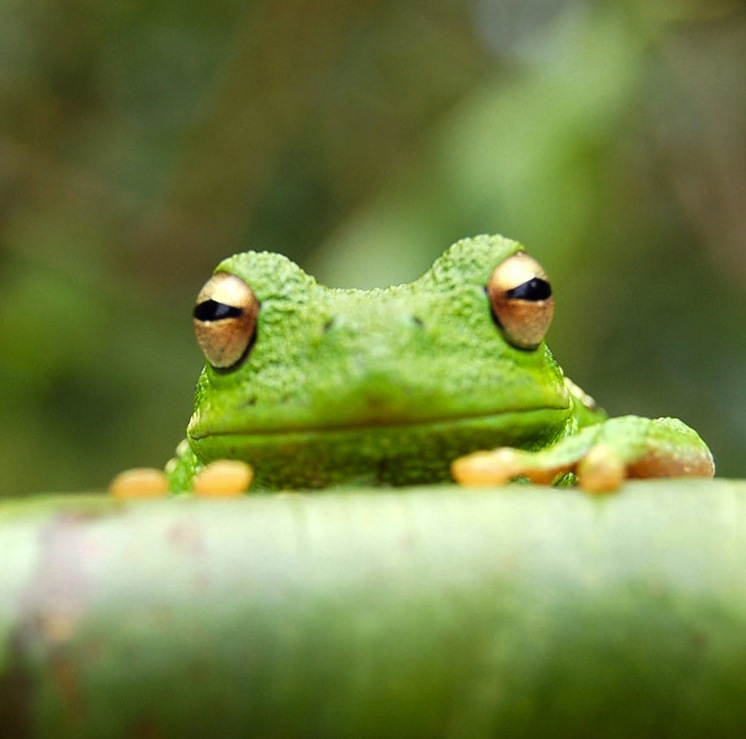
\includegraphics[width=\linewidth,height=7cm]{frog}
\captionof{figure}{This is a figure in the appendix}
\end{center}

\section{Secondly}


\begin{center}
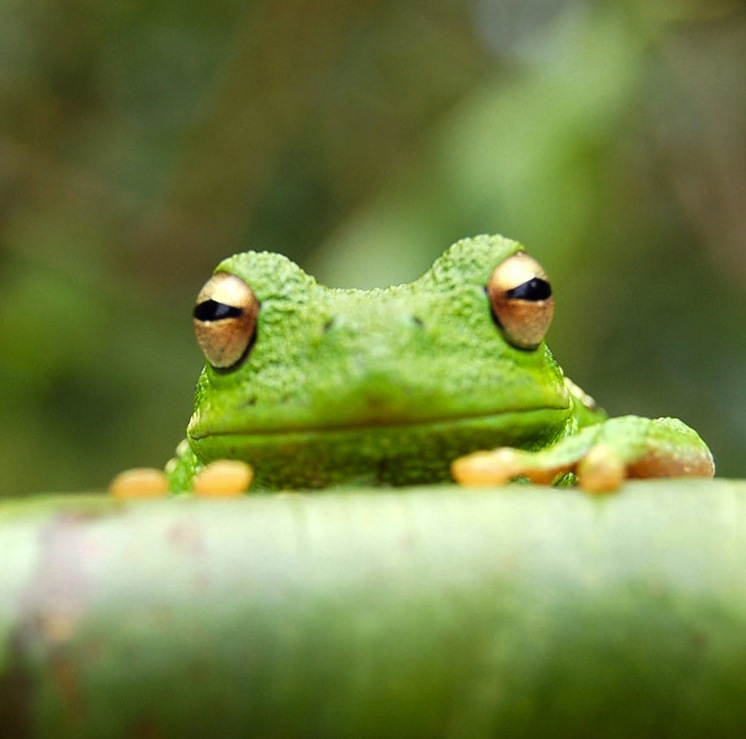
\includegraphics[width=\linewidth,height=7cm]{frog}
\captionof{figure}{This is a figure in the appendix}
\end{center}

\end{appendixbox}

\begin{appendixbox}
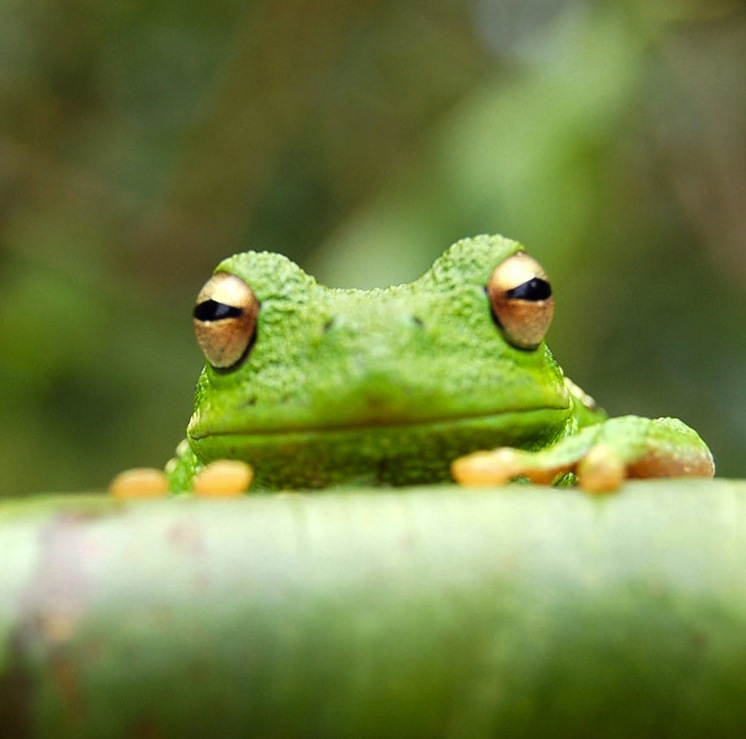
\includegraphics[width=\linewidth,height=7cm]{frog}
\captionof{figure}{This is a figure in the appendix}
\end{appendixbox}